\documentclass[12pt]{article}
\usepackage{geometry} % Pour passer au format A4
\geometry{hmargin=1cm, vmargin=1cm} % 

% Page et encodage
\usepackage[T1]{fontenc} % Use 8-bit encoding that has 256 glyphs
\usepackage[english,french]{babel} % Français et anglais
\usepackage[utf8]{inputenc} 

\usepackage{lmodern}
\setlength\parindent{0pt}

% Graphiques
\usepackage{graphicx,float,grffile}

% Maths et divers
\usepackage{amsmath,amsfonts,amssymb,amsthm,verbatim}
\usepackage{multicol,enumitem,url,eurosym,gensymb}

% Sections
\usepackage{sectsty} % Allows customizing section commands
\allsectionsfont{\centering \normalfont\scshape}

% Tête et pied de page

\usepackage{fancyhdr} 
\pagestyle{fancyplain} 

\fancyhead{} % No page header
\fancyfoot{}

\renewcommand{\headrulewidth}{0pt} % Remove header underlines
\renewcommand{\footrulewidth}{0pt} % Remove footer underlines

\newcommand{\horrule}[1]{\rule{\linewidth}{#1}} % Create horizontal rule command with 1 argument of height

%----------------------------------------------------------------------------------------
%	Début du document
%----------------------------------------------------------------------------------------

\begin{document}

%----------------------------------------------------------------------------------------
% RE-DEFINITION
%----------------------------------------------------------------------------------------
% MATHS
%-----------

\newtheorem{Definition}{Définition}
\newtheorem{Theorem}{Théorème}
\newtheorem{Proposition}{Propriété}

% MATHS
%-----------
\renewcommand{\labelitemi}{$\bullet$}
\renewcommand{\labelitemii}{$\circ$}
%----------------------------------------------------------------------------------------
%	Titre
%----------------------------------------------------------------------------------------

\setlength{\columnseprule}{0pt}

\section*{DM1 - Statistiques}
\horrule{2px}

\subsection*{BFM}

\begin{multicols}{2}
En regardant l'information, \textsc{M. Lafond} se rend compte que certains journalistes de \textsc{BFM} ne sont pas très bons en mathématiques.\\
C'est à toi de corriger l'erreur. 

\begin{figure}[H]
	\centering
	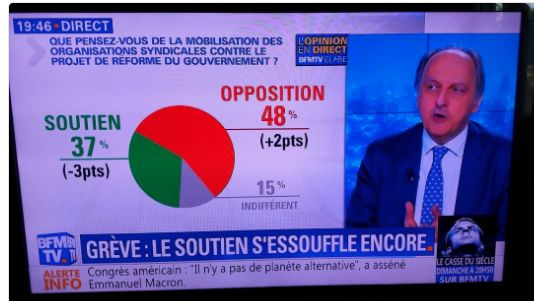
\includegraphics[width=\linewidth]{3x1-statistiques/sources/bfm.jpg}
\end{figure}

\end{multicols}

\begin{itemize}
	\item[1.] Le diagramme circulaire était-il une représentation graphique adaptée aux données ? \textbf{(Justifier !)}
	\item[2.] En un coup d'œil, il y a une erreur. Laquelle ?
	\item[3.] Faite un tableau avec les pourcentages et les angles du diagramme.
	\item[4.] Représenter les données dans un diagramme circulaire, mais cette fois juste.
\end{itemize}	

\subsection*{Liberation}

\begin{multicols}{2}

En regardant l'information, \textsc{M. Lafond} se rend compte que certains journalistes de \textsc{Liberation} ne sont pas très bons en mathématiques.\\
C'est à toi de corriger l'erreur. 

\begin{figure}[H]
	\centering
	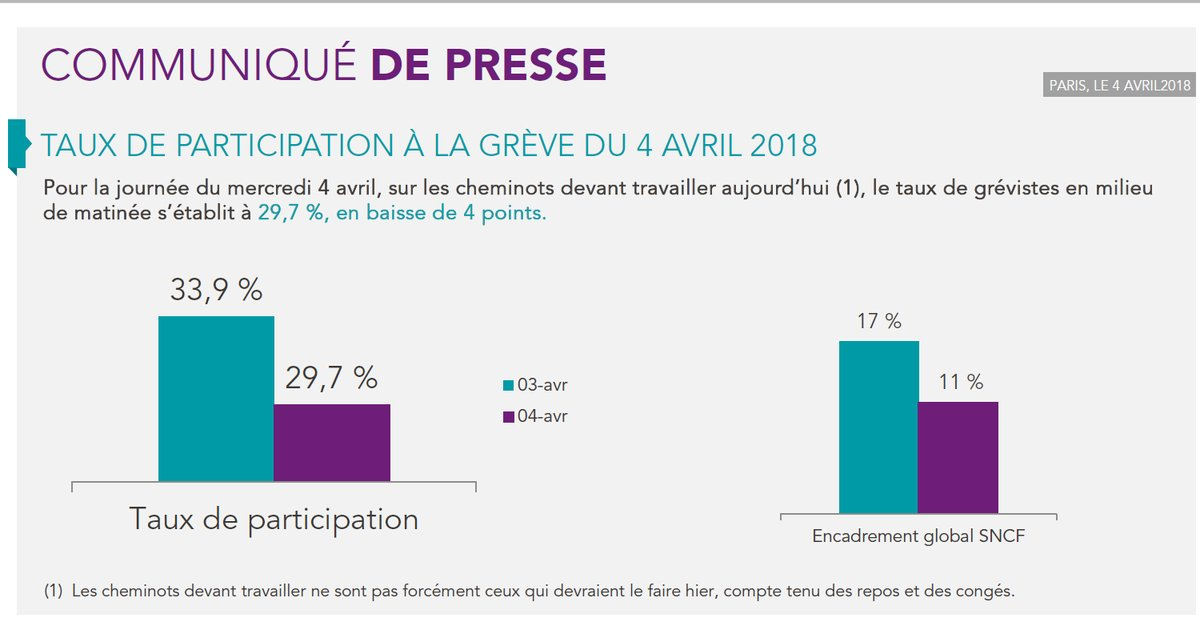
\includegraphics[width=\linewidth]{3x1-statistiques/sources/liberation.jpg}
\end{figure}

\end{multicols}

\begin{itemize}
	\item[1.] Un des deux graphiques est faux et ne respecte pas le principe de proportionnalité sur l'echelle des ordonnées. Lequel ? \textbf{(Justifier !)}
	\item[2.] Représenter les \textbf{deux} graphiques avec des diagrammes en bâton, mais cette fois justes.
\end{itemize}	

\subsection*{Bonus}

Bravo, vous êtes meilleurs en mathématiques qu'un journaliste de BFM et de Liberation. À moins que... \\
\textit{Pensez-vous que le graphique soit volontairement faux ou bien était-ce de l'incompétence ?} (2/3 lignes.)

\end{document}